\documentclass[11pt,a4paper]{article}
\usepackage[utf8]{inputenc}
\usepackage[T1]{fontenc}
\usepackage{lmodern}
\usepackage{microtype}
\usepackage[a4paper,margin=2.15cm,headheight=15pt]{geometry}
\usepackage{amsmath,amssymb,mathtools,bm}
\usepackage{booktabs,tabularx,longtable,array,multirow}
\usepackage{enumitem}
\usepackage{graphicx}
\usepackage{xcolor}
\usepackage{tikz}
\usetikzlibrary{arrows.meta,positioning,calc,fit,shapes.geometric,decorations.pathreplacing}
\usepackage{tcolorbox}
\tcbuselibrary{breakable,skins}
\usepackage{listings}
\usepackage{fancyhdr}
\usepackage{hyperref}
\usepackage[nameinlink,noabbrev]{cleveref}
\usepackage[numbers,sort&compress]{natbib}
\usepackage{caption}
\usepackage{subcaption}
\usepackage{float}
\usepackage{setspace}

\definecolor{Navy}{HTML}{14243E}
\definecolor{Blue}{HTML}{1C6F9F}
\definecolor{Sky}{HTML}{D9ECF8}
\definecolor{Gold}{HTML}{D69B2D}
\definecolor{Warm}{HTML}{FFF5DF}
\definecolor{Red}{HTML}{A83E45}
\definecolor{Green}{HTML}{31735C}
\definecolor{LightGray}{HTML}{F2F4F7}
\definecolor{MidGray}{HTML}{5D6D84}

\hypersetup{
  colorlinks=true,
  linkcolor=Navy,
  citecolor=Blue,
  urlcolor=Blue,
  pdftitle={Geometric Path Memory},
  pdfauthor={Guillaume Harbonnier}
}

\pagestyle{fancy}
\fancyhf{}
\lhead{Geometric Path Memory}
\rhead{MMALS Engineering Package}
\cfoot{\thepage}

\newcommand{\rhoop}{\bm{\rho}}
\newcommand{\Tr}{\operatorname{Tr}}
\newcommand{\norm}[1]{\left\lVert #1 \right\rVert}
\newcommand{\dd}{\mathrm{d}}
\newcommand{\parallelpart}{\parallel}
\newcommand{\perppart}{\perp}
\newcommand{\R}{\mathbb{R}}
\newcommand{\C}{\mathbb{C}}
\newcommand{\Hspace}{\mathcal{H}}

\newtcolorbox{executivebox}{
  breakable, enhanced, colback=Sky, colframe=Blue,
  title=Executive point, fonttitle=\bfseries, boxrule=0.8pt, arc=2mm
}
\newtcolorbox{kidbox}{
  breakable, enhanced, colback=Warm, colframe=Gold,
  title=12-year-old view, fonttitle=\bfseries, boxrule=0.8pt, arc=2mm
}
\newtcolorbox{engineerbox}{
  breakable, enhanced, colback=LightGray, colframe=Navy,
  title=Engineer view, fonttitle=\bfseries, boxrule=0.8pt, arc=2mm
}
\newtcolorbox{criticalbox}{
  breakable, enhanced, colback=red!3, colframe=Red,
  title=Critical correction, fonttitle=\bfseries, boxrule=0.8pt, arc=2mm
}
\newtcolorbox{researchbox}{
  breakable, enhanced, colback=green!4, colframe=Green,
  title=Research hypothesis to validate, fonttitle=\bfseries, boxrule=0.8pt, arc=2mm
}

\lstset{
  basicstyle=\ttfamily\small,
  frame=single,
  rulecolor=\color{MidGray},
  backgroundcolor=\color{LightGray},
  breaklines=true,
  columns=fullflexible,
  showstringspaces=false,
  keywordstyle=\color{Blue}\bfseries,
  commentstyle=\color{Green},
  stringstyle=\color{Red}
}

\title{\vspace{-1.2cm}\textbf{Geometric Path Memory}\\[0.3cm]
\Large From Lindblad-Uhlmann Open Quantum Dynamics to MMALS and Engineering Systems}
\author{Guillaume Harbonnier\\\small Critical review, corrected mathematical framing, interactive experiments, and implementation blueprint}
\date{25 July 2026\\\small Version 0.1.0}

\begin{document}
\maketitle
\begin{center}
\begin{minipage}{0.92\textwidth}
\small
\textbf{Suggested GitHub repository:} \texttt{mmals-geometric-path-memory}\\
\textbf{Short description:} A reproducible engineering study and interactive lab translating Lindblad-Uhlmann open-system geometry into path-sensitive continual learning, domain-shift diagnostics, and evidence-aware AI systems.
\end{minipage}
\end{center}

\begin{executivebox}
This package extracts a valuable idea from the reviewed manuscript: the current state of a system and the path used to reach it are different sources of information. It then corrects several mathematical overstatements and turns the remaining structure into an engineering program. The priority application is MMALS: distinguish reorientation inside an existing regime from structural change that may justify rerouting, host creation, host splitting, replay protection, or human review.
\end{executivebox}

\vspace{0.2cm}
\noindent\textbf{Scientific status.} This document is neither an endorsement nor a rejection of the source manuscript \citep{elmorsalani2026}. It separates established background, claims made in that manuscript, identified proof obligations, and new engineering hypotheses. Numerical demonstrations support reproducibility and intuition; they do not replace mathematical proof or physical validation.

\tableofcontents
\newpage

\section{Decision summary}

\subsection{What should be retained}

The reviewed work combines GKSL/Lindblad dynamics, coadjoint-orbit geometry, and Uhlmann parallel transport \citep{lindblad1976,gorini1976,uhlmann1986,uhlmann1991,souriau1969}. Its most reusable insights are:

\begin{enumerate}[label=\arabic*.]
  \item Separate motion that preserves structural invariants from motion that changes them.
  \item Do not confuse an endpoint statistic with a path-dependent statistic.
  \item Measure whether operations commute; order sensitivity can reveal hidden interference.
  \item Treat symmetry breaking as an observable structural event, not merely as scalar degradation.
\end{enumerate}

\subsection{What must be corrected}

Before using the manuscript as a formal foundation, at least five points require revision:

\begin{enumerate}[label=\arabic*.]
  \item For degenerate spectra, tangency must be expressed with spectral projectors, not only diagonal entries.
  \item The dissipator is not generically a purely normal vector; it may contain tangent and transverse components.
  \item A coadjoint orbit fixes the full spectrum; an entropy level set usually does not.
  \item A path-dependent holonomy is a compressed signature, not a lossless chronological ledger.
  \item The proposed curvature ``if and only if'' statement requires a more complete proof and explicit counterexample search.
\end{enumerate}

\subsection{Recommended action}

\begin{researchbox}
Create a new MMALS research track called \textbf{MMALS-Holo: Path-Sensitive Geometric Memory for Continual Learning}. Use normalized representation covariances as density-like operators, measure tangent and transverse evolution, perform curriculum-order experiments, and compare predictive power for future forgetting against MMD, Fisher-Rao/Bures, router energy, and standard representation-similarity baselines.
\end{researchbox}

\section{The idea at three levels}

\subsection{The 12-year-old view}

\begin{kidbox}
Imagine a marble inside a set of transparent nested shells. A gentle motor can move the marble around on the same shell. A different machine can push it through one shell into another. Looking only at the marble's final position may not tell you which machines acted, or in which order. Turning first and squeezing second can produce a different result from squeezing first and turning second.

For MMALS, each specialist is like a learned shell. A small turn means the specialist can adapt. A strong push through shells may mean that the system needs a new specialist, must divide an existing one, or must protect old knowledge before learning more.
\end{kidbox}

\subsection{The engineer view}

\begin{engineerbox}
Represent the system by a positive, trace-normalized matrix $\rho_t$. Its eigenvectors encode principal directions; its eigenvalues encode how capacity, variance, or probability is distributed across those directions. A local change $\Delta\rho_t$ can be decomposed relative to the current spectral blocks:
\[
\Delta\rho_t = \Delta\rho_t^{\parallel} + \Delta\rho_t^{\perp}.
\]
The cross-block part is tangent to the unitary orbit. The block-diagonal part changes spectral structure or acts inside degenerate subspaces. Separately, compare compositions $A\circ B$ and $B\circ A$. A large endpoint gap indicates order-sensitive interference that a scalar endpoint KPI can miss.
\end{engineerbox}

\subsection{The mathematical view}

Let $\rhoop$ be a full-rank density operator on an $n$-dimensional Hilbert space. The unitary group acts by conjugation,
\[
\rhoop \mapsto U\rhoop U^\dagger.
\]
The corresponding coadjoint orbit contains operators with the same spectrum. Its tangent space can be written
\[
T_{\rhoop}\mathcal{O}_{\rhoop}=\{-i[K,\rhoop] : K=K^\dagger\}.
\]
Under GKSL dynamics,
\begin{equation}
\dot{\rhoop}=-i[H,\rhoop]+\sum_k\gamma_k\left(L_k\rhoop L_k^\dagger-\frac12\{L_k^\dagger L_k,\rhoop\}\right),
\label{eq:gksl}
\end{equation}
we denote the Hamiltonian term by $X_H$ and the dissipative term by $X_D$. The Hamiltonian term is orbit-tangent. The dissipative term must be decomposed rather than automatically identified with the normal space.

\section{Reviewed manuscript: contribution map}

The manuscript \citep{elmorsalani2026} proposes a synthesis with four principal claims:

\begin{enumerate}[label=\textbf{C\arabic*.}]
  \item A geometric obstruction prevents generic dissipative paths from being represented by purely unitary horizontal lifts.
  \item Uhlmann curvature encodes the interaction between coherent and dissipative motion.
  \item Entropy production and transverse motion share a geometric origin.
  \item Dissipation can reduce a non-Abelian stabilizer, for example $U(2)$ to $U(1)\times U(1)$ in a qutrit example.
\end{enumerate}

The work also sketches an ancilla-assisted interferometric readout under noise. The conceptual direction is interesting because it asks for an operational observable rather than stopping at geometric language. The practical claims, however, require a stronger experimental protocol, a complete noise budget, identifiability analysis, and a clearer distinction between the proposed observable and existing mixed-state phase schemes.

\begin{table}[H]
\centering
\caption{Separation of knowledge layers}
\begin{tabularx}{\textwidth}{p{0.19\textwidth} X X}
\toprule
\textbf{Layer} & \textbf{Content} & \textbf{Status in this package} \\
\midrule
Established background & GKSL dynamics, density matrices, unitary orbits, Uhlmann transport, Bures geometry & Used as standard theory with references \\
Source claims & Obstruction theorem, curvature-dissipation equivalence, thermodynamic leaf identification, gauge reduction & Reviewed critically; not assumed proven \\
Engineering proposal & Covariance density operators, tangent/transverse MMALS diagnostics, curriculum-order metrics & New hypotheses with executable validation plan \\
\bottomrule
\end{tabularx}
\end{table}


\section{Core geometric machinery}

\subsection{Density matrices as structured states}

A density matrix satisfies
\[
\rhoop=\rhoop^\dagger,\qquad \rhoop\succeq 0,\qquad \Tr(\rhoop)=1.
\]
Its spectral decomposition is
\[
\rhoop=\sum_a \lambda_a P_a,
\]
where $P_a$ projects onto an eigenspace, possibly of dimension greater than one. The spectrum encodes mixedness and invariant information under unitary conjugation. The eigenvectors encode orientation of the spectral subspaces.

The von Neumann entropy is
\begin{equation}
S(\rhoop)=-\Tr(\rhoop\log\rhoop)=-\sum_i\lambda_i\log\lambda_i.
\label{eq:entropy}
\end{equation}
It depends on the spectrum but does not uniquely identify it for general dimension.

\subsection{Orbit-preserving motion}

For a Hermitian generator $H$,
\[
X_H(\rhoop)=-i[H,\rhoop].
\]
This changes eigenvectors while preserving eigenvalues. Consequently,
\[
\frac{\dd}{\dd t}S(\rhoop(t))=0
\]
for a purely Hamiltonian trajectory. The geometric intuition is rotation along a fixed spectral leaf.

\subsection{Dissipative motion}

The dissipator in \cref{eq:gksl} can change populations, coherences, rank, and asymptotic state. A qubit amplitude-damping channel gives a familiar example. In Bloch coordinates,
\[
(x,y,z)\mapsto \left(\sqrt{1-p}\,x,\sqrt{1-p}\,y,(1-p)z+p\right).
\]
It is anisotropic: transverse components contract, while the state is translated toward the ground-state pole.

\begin{figure}[H]
\centering
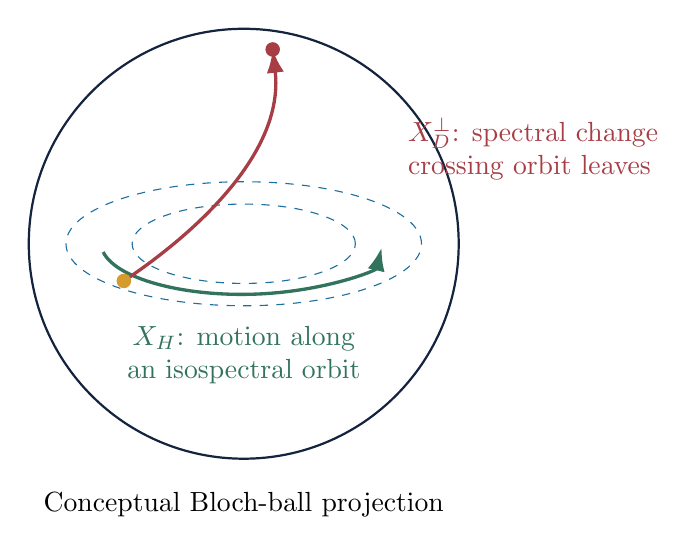
\begin{tikzpicture}[scale=1.05,>=Latex]
  \draw[thick,Navy] (0,0) circle (2.6);
  \draw[Blue,dashed] (0,0) ellipse (2.15 and 0.75);
  \draw[Blue,dashed] (0,0) ellipse (1.35 and 0.48);
  \draw[->,very thick,Green] (-1.7,-0.1) arc[start angle=190,end angle=355,x radius=1.7,y radius=.62];
  \draw[->,very thick,Red] (-1.45,-0.45) .. controls (-0.7,0.05) and (0.5,1.05) .. (0.35,2.35);
  \node[Green,align=center] at (0,-1.35) {$X_H$: motion along\\an isospectral orbit};
  \node[Red,align=left] at (3.5,1.15) {$X_D^{\perp}$: spectral change\\crossing orbit leaves};
  \fill[Gold] (-1.45,-0.45) circle (2.5pt);
  \fill[Red] (0.35,2.35) circle (2.5pt);
  \node at (0,-3.15) {Conceptual Bloch-ball projection};
\end{tikzpicture}
\caption{Orbit-tangent and transverse intuition. A general dissipator can contain both components.}
\label{fig:bloch}
\end{figure}

\subsection{Purification and Uhlmann transport}

A full-rank density operator can be represented by an amplitude $W$ such that
\[
\rhoop=WW^\dagger.
\]
The representation is gauge-redundant because $WV$ gives the same density operator for any unitary $V$. Uhlmann parallel transport selects a horizontal relation between neighboring amplitudes \citep{uhlmann1986,uhlmann1991}. For a smooth horizontal lift, the manuscript uses a Hermitian generator $G$ satisfying the Lyapunov equation
\begin{equation}
G\rhoop+\rhoop G=\dot{\rhoop}.
\label{eq:lyapunov}
\end{equation}
In the eigenbasis of $\rhoop$,
\begin{equation}
G_{ij}=\frac{\dot\rho_{ij}}{\lambda_i+\lambda_j},
\label{eq:g_elements}
\end{equation}
provided the state is full rank.

For a discretized path $\rho_0,\ldots,\rho_N$, a practical parallel-alignment rule uses the polar decomposition
\[
\sqrt{\rho_{k+1}}\sqrt{\rho_k}=U_k P_k,
\]
and accumulates the unitary factors $U_k$. For a closed path, their ordered product is a discrete holonomy estimate. It is path-dependent but not a complete, injective encoding of every possible path.

\section{Mathematical corrections and proof obligations}

\subsection{Degenerate spectra require spectral blocks}

\begin{criticalbox}
The condition ``all diagonal elements vanish in an eigenbasis'' is sufficient only in the non-degenerate case. When eigenvalues are degenerate, the basis inside each degenerate eigenspace is not unique. A basis-dependent diagonal test cannot characterize tangency.
\end{criticalbox}

Let
\[
\rhoop=\sum_a\lambda_a P_a
\]
with distinct eigenvalues indexed by $a$. A Hermitian velocity $X$ decomposes as
\begin{align}
X^{\perp} &= \sum_a P_a X P_a, \\
X^{\parallel} &= \sum_{a\neq b}P_a X P_b.
\label{eq:block_decomp}
\end{align}
The cross-block component belongs to the image of the commutator map and is tangent to the unitary orbit. The block-diagonal component is the obstruction to representing the full velocity as $-i[K,\rhoop]$. In a non-degenerate spectrum, each $P_a$ has rank one, and the criterion reduces to vanishing diagonal entries.

\subsection{The dissipator is not automatically normal}

A general Lindblad dissipator can rotate coherences and change eigenvalues simultaneously. Therefore,
\[
X_D=X_D^{\parallel}+X_D^{\perp}.
\]
This distinction is operationally important: ``dissipation exists'' and ``spectral structure changes'' are not equivalent statements. A dephasing channel, an amplitude-damping channel, and an engineered reservoir can have very different tangent/transverse compositions.

\subsection{Entropy leaves are coarser than spectral orbits}

\begin{criticalbox}
A unitary orbit fixes the complete spectrum. Entropy is only one scalar function of that spectrum. Therefore, an orbit lies inside an entropy level set, but a general entropy level set contains many different orbits.
\end{criticalbox}

The correct relation is
\[
\mathcal O_{\rhoop}\subseteq \{\sigma:S(\sigma)=S(\rhoop)\},
\]
with equality only in special low-dimensional or constrained cases. This correction matters because a nonzero entropy derivative is a sufficient indicator of leaving the orbit, but a zero entropy derivative does not guarantee that the spectrum is unchanged.

\subsection{A horizontal-unitary contradiction must be scoped carefully}

The manuscript shows that a horizontal velocity of the particular form $\dot W=-i\Omega W$ vanishes under its conventions. This is not by itself a dissipation-specific theorem. The meaningful result is narrower: horizontal transport of amplitudes is not generally equivalent to applying an active unitary on the left, even when the base motion is unitary. A revised theorem should state exactly which action, bundle convention, and connection are used.

\subsection{Curvature equivalence requires counterexample search}

The proposed identity between nonzero mixed curvature and active spectral-coherence distortion is plausible as a diagnostic direction but not established merely by saying that two terms are structurally mismatched. A publishable proof should include:

\begin{enumerate}
  \item a coordinate-independent derivation of the connection and curvature;
  \item a precise definition of the base Lie bracket and lifted generators;
  \item proof of necessity and sufficiency, or a weaker one-direction implication;
  \item symbolic checks in dimension two and three;
  \item numerical searches for cancellation counterexamples;
  \item explicit treatment of degeneracy crossings and rank-deficient boundaries.
\end{enumerate}

\subsection{Holonomy is compressed memory, not full history}

Two different paths can yield the same holonomy. Gauge-invariant observables may further compress the result. The defensible statement is:

\begin{quote}
Holonomy can retain path-dependent information not contained in the instantaneous density matrix, but it is not generally a lossless or uniquely decodable chronological record.
\end{quote}


\section{Corrected engineering abstraction}

The physics suggests a reusable systems pattern without claiming physical equivalence.

\subsection{State, invariants, and regimes}

Choose a structured state descriptor $Q_t$ that is positive and normalized:
\[
Q_t\succeq0,\qquad \Tr(Q_t)=1.
\]
Examples include:

\begin{itemize}
  \item normalized latent covariance for a neural-network host;
  \item normalized error covariance for an EO/IR estimator;
  \item normalized graph diffusion or risk operator for identity fraud;
  \item normalized evidence-transition matrix for release governance.
\end{itemize}

The eigenstructure of $Q_t$ separates orientation and spectral allocation. A regime is not defined by a single scalar; it is represented by a neighborhood in a structured state space plus operational constraints.

\subsection{Local decomposition}

For a finite difference
\[
\Delta Q_t=Q_{t+1}-Q_t,
\]
compute spectral projectors $P_a$ of $Q_t$ and define
\begin{align}
\Delta Q_t^{\perp}&=\sum_aP_a\Delta Q_tP_a,\\
\Delta Q_t^{\parallel}&=\Delta Q_t-\Delta Q_t^{\perp}.
\end{align}
A simple normalized structural-change score is
\begin{equation}
r_{\perp}(t)=\frac{\norm{\Delta Q_t^{\perp}}_F}{\norm{\Delta Q_t^{\parallel}}_F+\norm{\Delta Q_t^{\perp}}_F+\epsilon}.
\label{eq:transverse_ratio}
\end{equation}

\subsection{Order sensitivity}

For two update operators $A$ and $B$, compare
\begin{align}
Q_{AB}&=(B\circ A)(Q_0),\\
Q_{BA}&=(A\circ B)(Q_0).
\end{align}
Candidate metrics include
\begin{align}
O_{\mathrm{end}}&=\norm{Q_{AB}-Q_{BA}}_F,\\
O_{\mathrm{map}}&=\norm{AB-BA}_F,\\
O_{\mathrm{task}}&=\left|\mathcal L(Q_{AB})-\mathcal L(Q_{BA})\right|.
\end{align}
The endpoint gap, map commutator, and task loss answer different questions and should be retained separately.

\subsection{Composite decision score}

A practical controller may combine geometry with established signals:
\begin{equation}
R_t=w_EE_t+w_UU_t+w_Tr_{\perp}(t)+w_OO_t+w_DD_t+w_CC_t,
\label{eq:control_score}
\end{equation}
where $E_t$ is routing energy, $U_t$ uncertainty, $O_t$ order sensitivity, $D_t$ drift evidence, and $C_t$ operational cost or constraint pressure. The weights must be calibrated on downstream outcomes, not selected only for geometric elegance.

\begin{figure}[H]
\centering
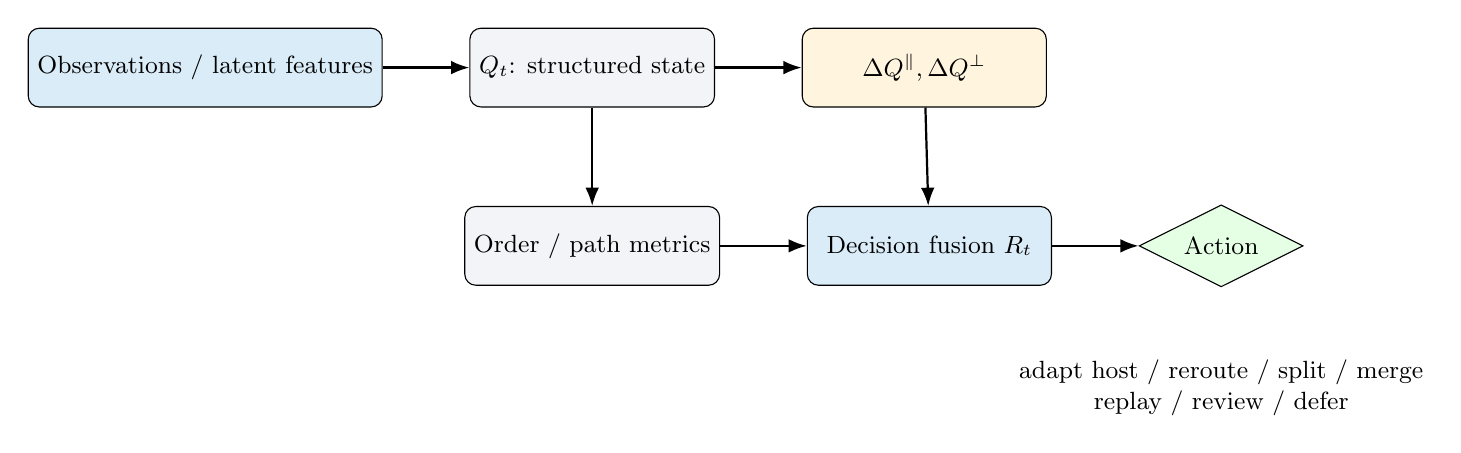
\begin{tikzpicture}[node distance=1.25cm and 1.1cm,>=Latex,every node/.style={font=\small}]
\node[draw,rounded corners,fill=Sky,minimum width=3.2cm,minimum height=1cm] (data) {Observations / latent features};
\node[draw,rounded corners,fill=LightGray,right=of data,minimum width=3.0cm,minimum height=1cm] (state) {$Q_t$: structured state};
\node[draw,rounded corners,fill=Warm,right=of state,minimum width=3.1cm,minimum height=1cm] (decomp) {$\Delta Q^{\parallel},\Delta Q^{\perp}$};
\node[draw,rounded corners,fill=LightGray,below=of state,minimum width=3.0cm,minimum height=1cm] (path) {Order / path metrics};
\node[draw,rounded corners,fill=Sky,right=of path,minimum width=3.1cm,minimum height=1cm] (decision) {Decision fusion $R_t$};
\node[draw,diamond,aspect=2.0,fill=green!10,right=of decision] (action) {Action};
\draw[->,thick] (data)--(state);
\draw[->,thick] (state)--(decomp);
\draw[->,thick] (state)--(path);
\draw[->,thick] (decomp)--(decision);
\draw[->,thick] (path)--(decision);
\draw[->,thick] (decision)--(action);
\node[align=center,below=0.8cm of action] {adapt host / reroute / split / merge\\replay / review / defer};
\end{tikzpicture}
\caption{Path-sensitive engineering control loop. Geometry augments rather than replaces domain evidence.}
\label{fig:control_loop}
\end{figure}

\section{Priority application: MMALS}

\subsection{Why the mapping is useful}

MMALS must discover, merge, split, and refine regimes without relying on a task identifier. Its central difficulty is deciding whether incoming data belongs to:

\begin{itemize}
  \item a known regime requiring plastic adaptation;
  \item a known regime seen under benign reorientation;
  \item a mixed or ambiguous region requiring multi-host routing;
  \item a genuinely new regime requiring structural expansion;
  \item a harmful transition causing forgetting or representational collapse.
\end{itemize}

The tangent/transverse decomposition gives a candidate diagnostic language for this decision.

\subsection{Density-like representation state}

For latent vectors $z_1,\ldots,z_m\in\R^d$, define
\begin{align}
\mu_t &= \frac1m\sum_{i=1}^m z_i,\\
\Sigma_t &= \frac{1}{m-1}\sum_{i=1}^m(z_i-\mu_t)(z_i-\mu_t)^\top,\\
\rhoop_t &= \frac{\Sigma_t+\epsilon I}{\Tr(\Sigma_t+\epsilon I)}.
\label{eq:mmals_density}
\end{align}
Alternative operators may be built from Fisher information, prototype Gram matrices, activation kernels, or class-conditional covariance. The covariance version is the simplest starting point because it is interpretable and computationally tractable.

\begin{table}[H]
\centering
\caption{Quantum-to-MMALS translation table}
\begin{tabularx}{\textwidth}{p{0.25\textwidth} X X}
\toprule
\textbf{Geometric concept} & \textbf{MMALS interpretation} & \textbf{Operational question} \\
\midrule
Eigenvectors & Principal latent directions & Did the representation mainly rotate? \\
Eigenvalues & Capacity or variance allocation & Did specialization or collapse redistribute capacity? \\
Isospectral motion & Reorientation inside a regime & Can the current host adapt safely? \\
Spectral-block motion & Structural regime change & Should the router create, split, merge, or protect a host? \\
Entropy & Effective latent diversity & Is diversity increasing, concentrating, or collapsing? \\
Path order & Curriculum/interference history & Does learning $A$ then $B$ differ from $B$ then $A$? \\
Holonomy-inspired metric & Compressed path signature & Is there useful history beyond endpoint accuracy? \\
\bottomrule
\end{tabularx}
\end{table}

\subsection{Controller design}

A possible host decision table is shown in \cref{tab:mmals_decisions}.

\begin{table}[H]
\centering
\caption{Illustrative MMALS actions}
\label{tab:mmals_decisions}
\begin{tabularx}{\textwidth}{p{0.16\textwidth} p{0.17\textwidth} p{0.18\textwidth} X}
\toprule
$r_\perp$ & Router confidence & Retention risk & Suggested action \\
\midrule
Low & High & Low & Adapt current host; monitor only \\
Low & Low & Medium & Soft multi-host routing; collect evidence \\
High & High prototype match & Medium & Reroute to known host or evaluate merge \\
High & Low & High & Create/split host; protected replay; human review \\
Any & Any & High order gap & Run curriculum permutation and interference tests \\
\bottomrule
\end{tabularx}
\end{table}

\subsection{MMALS-Holo experiment matrix}

\begin{longtable}{p{0.16\textwidth} p{0.21\textwidth} p{0.25\textwidth} p{0.27\textwidth}}
\caption{Research protocol}\label{tab:protocol}\\
\toprule
\textbf{Axis} & \textbf{Values} & \textbf{Measurements} & \textbf{Purpose} \\
\midrule
\endfirsthead
\toprule
\textbf{Axis} & \textbf{Values} & \textbf{Measurements} & \textbf{Purpose} \\
\midrule
\endhead
Dataset & RotatedMNIST, PermutedMNIST, SplitCIFAR-10/100, CORe50 & Accuracy, average forgetting, backward transfer, calibration & Cover benign rotation, permutation, class split, and real drift \\
Order & Original, reversed, random permutations, adversarial curricula & Endpoint gap, commutator proxy, retention delta & Test whether path metrics explain curriculum sensitivity \\
State operator & Covariance, Fisher, prototype Gram, class-conditional blocks & $r_\perp$, entropy, Bures/Fisher-Rao, MMD & Identify the most predictive geometry \\
Router & Oracle, clustering, energy router, MMALS router & routing accuracy, host utilization, false split/merge & Separate geometry quality from router quality \\
Memory & None, replay, EWC, functional memory & forgetting and memory cost & Test whether path alerts improve protection decisions \\
Ablation & No geometry, permuted blocks, random projectors & predictive value and false alarms & Detect spurious correlation \\
\bottomrule
\end{longtable}

\subsection{Primary falsifiable hypotheses}

\begin{researchbox}
\textbf{H1 - Structural prediction.} The integrated transverse energy
\[
E_\perp=\sum_t\norm{\Delta\rhoop_t^\perp}_F
\]
predicts future forgetting better than entropy change alone.

\textbf{H2 - Order sensitivity.} The endpoint order gap between curriculum permutations predicts asymmetric backward transfer.

\textbf{H3 - Decision value.} A router using geometry only when it changes an operational action improves retention-cost trade-offs compared with an always-on geometric penalty.

\textbf{H4 - Non-equivalence.} MMD, Bures/Fisher-Rao, and tangent/transverse scores provide complementary rather than redundant signals.
\end{researchbox}


\section{Application to EO/IR domain shift}

For EO/IR geolocation and tracking, let $\Sigma_t$ represent an error covariance over position, attitude, timing, boresight, terrain intersection, or fused state. Normalize it to $Q_t$. Then:

\begin{itemize}
  \item a rotation of uncertainty axes caused by a platform maneuver can be mainly orientation change;
  \item growth of one eigenvalue due to blur, thermal noise, poor texture, or degraded GNSS is structural spectral change;
  \item two fault sequences can end with similar CEP50 yet have different recoverability and residual bias;
  \item a path metric can complement Fisher information, Cramer-Rao bounds, CEP50, and MMD-based sample shift.
\end{itemize}

\subsection{Relationship to Fisher-Rao and MMD}

\begin{table}[H]
\centering
\caption{Complementary domain-shift lenses}
\begin{tabularx}{\textwidth}{p{0.2\textwidth} X X}
\toprule
\textbf{Tool} & \textbf{What it measures} & \textbf{Engineering use} \\
\midrule
MMD \citep{gretton2012} & Difference between sample distributions in an RKHS & Detect that observed data changed \\
Fisher-Rao / Bures \citep{amari2016,hubner1992} & Geometric displacement inside a statistical model/state manifold & Measure model-relative distinguishability and uncertainty movement \\
Tangent/transverse split & Orientation change versus spectral-block redistribution & Classify benign reorientation versus structural degradation \\
Path-order metric & Non-commutativity of fault or adaptation sequences & Detect history effects hidden by similar endpoints \\
\bottomrule
\end{tabularx}
\end{table}

A useful EO/IR study would simulate identical final covariance traces produced by different sequences: blur then stabilization, stabilization then blur, timing drift then map correction, and reversed order. The question is not whether a quantum holonomy literally occurs, but whether an ordered geometric signature improves failure diagnosis or recovery prediction.

\section{Application to identity and credential fraud}

Identity fraud is path-dependent by nature. A final profile can appear individually plausible while its construction history is anomalous. Let $G_t$ be a temporal identity graph and let $Q_t$ summarize diffusion, reuse, or risk concentration across identity, device, credential, telco, document, and biometric nodes.

Candidate path-sensitive signals include:

\begin{itemize}
  \item order of address, device, SIM, and document changes;
  \item repeated transitions between enrollment and recovery channels;
  \item credential reuse followed by biometric replacement;
  \item graph-community changes before and after high-risk events;
  \item exclusion trajectories in which legitimate citizens are repeatedly rejected by an unsuitable process.
\end{itemize}

A combined risk score can be written
\[
R_t=w_sS_{\mathrm{sup}}+w_aS_{\mathrm{anom}}+w_gS_{\mathrm{graph}}+w_pS_{\mathrm{path}}+w_dS_{\mathrm{drift}}.
\]
The path component should be explainable as event sequences, graph motifs, and counterfactual order tests. It must not become an opaque justification for surveillance or exclusion.

\begin{engineerbox}
The useful lesson is not ``use quantum fraud detection.'' It is ``do not score only the final snapshot.'' Maintain a versioned event graph, compare plausible construction paths, identify non-commuting high-risk transitions, and preserve human review for adverse decisions.
\end{engineerbox}

\section{Application to STRAT-Q and Test Authority}

Two releases can have similar final dashboards while possessing very different evidence histories. A release that accumulated representative evidence progressively is not equivalent to one that reached the same KPI through late waivers, partial reruns, and non-representative environments.

Define a release state $Q_t$ from requirements, risks, test evidence, environment representativity, defect transitions, and decision confidence. Path-aware governance asks:

\begin{itemize}
  \item Did the evidence mature before or after critical design decisions?
  \item Were defects closed before or after environment changes?
  \item Did a waiver precede a test reduction, or did a test reduction create the waiver need?
  \item Were requirements changed after evidence was generated?
  \item Can the release state be replayed from versioned events?
\end{itemize}

This maps naturally to the planned OTEL spec-to-evidence backbone, XES/OCEL event models, XRAY evidence, and reproducible decision packages.

\subsection{C-level wording}

Avoid quantum terminology in executive governance. Use:

\begin{quote}
\textbf{Path-aware decision and evidence integrity:} release confidence considers not only current KPI values, but also the sequence, provenance, representativity, and reversibility of the evidence that produced them.
\end{quote}

\section{Quantum engineering learning path}

This topic is valuable for the user's three-to-five-year quantum roadmap because it connects linear algebra, Lie groups, differential geometry, quantum information, and open-system control.

\subsection{Prerequisite chain}

\begin{enumerate}[label=\arabic*.]
  \item Complex vector spaces, Hermitian matrices, eigenvalues, tensor products.
  \item Density matrices, partial trace, purification, completely positive maps.
  \item Lie groups and Lie algebras: $U(n)$, commutators, adjoint and coadjoint actions.
  \item Differential geometry: tangent spaces, bundles, connections, curvature, holonomy.
  \item Information geometry: Fisher metric, Bures metric, distinguishability.
  \item Open quantum dynamics: GKSL generators, decoherence, engineered reservoirs.
  \item Numerical methods: matrix exponentials, Lyapunov equations, polar decompositions.
\end{enumerate}

\subsection{Full practical lab}

The repository contains a first notebook. The next physical-computing lab should include:

\begin{enumerate}
  \item exact and numerical amplitude damping of a qubit;
  \item Bloch-ball trajectory and entropy evolution;
  \item tangent/transverse projection in the instantaneous eigenbasis;
  \item solution of \cref{eq:lyapunov};
  \item closed loops with discrete Uhlmann transport;
  \item a qutrit with controlled degeneracy splitting;
  \item sensitivity to ancilla noise and finite sampling;
  \item symbolic and numerical tests of proposed curvature identities.
\end{enumerate}

\section{Interactive tools}

Two standalone browser tools are included.

\subsection{Open Quantum Order Lab}

\texttt{tools/open\_quantum\_order\_lab.html} visualizes a qubit in the Bloch $x$-$z$ projection. Sliders control the initial state, rotation, damping probability, and trajectory resolution. It compares rotation-then-damping with damping-then-rotation and reports:

\begin{itemize}
  \item trace-distance order gap;
  \item final entropy in both orders;
  \item initial purity;
  \item final Bloch vectors;
  \item exportable JSON evidence.
\end{itemize}

\subsection{MMALS Path Memory Lab}

\texttt{tools/mmals\_path\_memory\_lab.html} uses a $2\times2$ covariance ellipse. Operation A rotates the representation. Operation B applies anisotropic scale and shear. It displays:

\begin{itemize}
  \item $A\rightarrow B$ and $B\rightarrow A$ ellipses;
  \item normalized endpoint gap;
  \item map commutator norm;
  \item tangent/transverse proxy ratio;
  \item entropy delta;
  \item a threshold-based MMALS action recommendation.
\end{itemize}

Both tools are dependency-free HTML files and can be opened offline.


\section{Repository architecture and reproducibility}

\begin{verbatim}
mmals-geometric-path-memory/
|-- README.md
|-- CITATION.cff
|-- LICENSE
|-- pyproject.toml
|-- Makefile
|-- docs/
|   |-- main.tex
|   |-- references.bib
|   `-- Geometric_Path_Memory.pdf
|-- notebooks/
|   |-- 01_open_quantum_geometry.ipynb
|   `-- 02_mmals_path_memory.ipynb
|-- tools/
|   |-- open_quantum_order_lab.html
|   `-- mmals_path_memory_lab.html
|-- src/mmals_path_memory/
|   |-- geometry.py
|   `-- mmals.py
|-- tests/
|-- scripts/
`-- .github/workflows/ci.yml
\end{verbatim}

\subsection{Core API}

\begin{lstlisting}[language=Python,caption={Core transition diagnosis}]
from mmals_path_memory.mmals import covariance_density, diagnose_transition

rho_before = covariance_density(features_before)
rho_after = covariance_density(features_after)
result = diagnose_transition(rho_before, rho_after)

print(result.transverse_ratio)
print(result.recommendation)
\end{lstlisting}

\subsection{Quality gates}

The CI pipeline should enforce:

\begin{itemize}
  \item unit tests for positivity, trace normalization, decomposition reconstruction, and transport unitarity;
  \item static validation of offline HTML assets;
  \item LaTeX compilation;
  \item artifact upload of the compiled report;
  \item no hidden dependency on the source PDF.
\end{itemize}

\section{Validation strategy}

\subsection{Mathematical validation}

\begin{enumerate}
  \item Derive the spectral-projector decomposition rigorously.
  \item Verify the commutator-image characterization under degeneracy.
  \item Check the horizontal-lift convention against standard Uhlmann formulations.
  \item Re-derive curvature expressions from the connection form.
  \item Construct symbolic counterexample searches for claimed equivalences.
\end{enumerate}

\subsection{Numerical validation}

\begin{enumerate}
  \item Compare exact qubit channels with numerical integration.
  \item Check convergence of discrete transport as path resolution increases.
  \item Test sensitivity near rank-deficient states.
  \item Bootstrap latent covariance estimates under finite data.
  \item Evaluate false regime-split alerts under pure rotations.
  \item Evaluate missed structural changes under trace-preserving anisotropic transformations.
\end{enumerate}

\subsection{Product and decision validation}

A geometric metric is valuable only if it changes a real decision and improves outcomes. For MMALS, the relevant utility function may be
\[
U=\alpha\,\mathrm{retention}+\beta\,\mathrm{transfer}-\gamma\,\mathrm{compute}-\delta\,\mathrm{memory}-\eta\,\mathrm{false\ splits}.
\]
For Test Authority, utility concerns escaped risk, evidence cost, cycle time, and decision confidence. For fraud, utility must include false accusations, exclusion risk, explainability, and human-review capacity.

\section{Risks and limitations}

\begin{enumerate}
  \item \textbf{Metaphor risk.} Quantum geometry can become decorative jargon. Every imported concept must correspond to a measurable engineering object and a falsifiable benefit.
  \item \textbf{Estimation risk.} Covariance operators are noisy in high dimension. Shrinkage, low-rank approximation, and confidence intervals are necessary.
  \item \textbf{Degeneracy instability.} Near-equal eigenvalues make spectral projectors sensitive. Use tolerances, subspace tracking, and perturbation analysis.
  \item \textbf{Computational cost.} Full $d\times d$ operators are expensive. Use sketches, block structure, prototypes, or low-rank factorizations.
  \item \textbf{Causal overreach.} A path metric can correlate with forgetting without causing it.
  \item \textbf{Decision harm.} In identity and workforce contexts, geometry must not automate adverse decisions without explainable evidence and human safeguards.
  \item \textbf{Source maturity.} The reviewed manuscript contains promising synthesis but unresolved mathematical claims.
\end{enumerate}

\section{Twelve-week implementation roadmap}

\begin{longtable}{p{0.10\textwidth} p{0.27\textwidth} p{0.29\textwidth} p{0.24\textwidth}}
\caption{Proposed execution plan}\label{tab:roadmap}\\
\toprule
\textbf{Weeks} & \textbf{Build} & \textbf{Experiment} & \textbf{Exit evidence} \\
\midrule
\endfirsthead
\toprule
\textbf{Weeks} & \textbf{Build} & \textbf{Experiment} & \textbf{Exit evidence} \\
\midrule
\endhead
1--2 & Finalize mathematical corrections and API & Qubit and synthetic covariance validation & Unit tests and reviewed derivation \\
3--4 & Integrate covariance-density hooks into MMALS & RotatedMNIST order permutations & Baseline comparison and false-alert analysis \\
5--6 & Add Fisher/Bures and MMD baselines & PermutedMNIST and SplitCIFAR-10 & Predictive value for forgetting \\
7--8 & Add router decision fusion & SplitCIFAR-100 and host split/merge ablations & Retention-cost Pareto curves \\
9--10 & Add low-rank approximation and calibration & CORe50 drift and finite-sample bootstrap & Scalability and confidence intervals \\
11 & EO/IR synthetic fault-sequence pilot & Same endpoint, different fault order & Diagnostic lift over CEP/Fisher/MMD alone \\
12 & Consolidate paper, package, and decision memo & Reproducibility rerun & Versioned release candidate \\
\bottomrule
\end{longtable}

\section{Conclusion}

The reviewed manuscript points toward a genuinely useful distinction: state and trajectory are not interchangeable. Its strongest formal claims need correction and proof reinforcement, especially around degeneracy, tangent/normal decomposition, entropy leaves, and curvature equivalence. Once corrected, the framework becomes a productive engineering research program.

The most immediate opportunity is MMALS-Holo. A normalized representation covariance can expose orientation and spectral allocation; local projectors can separate tangent-like adaptation from structural change; operation-order tests can quantify curriculum interference; and these signals can be evaluated against real retention and cost outcomes. EO/IR, identity fraud, and Test Authority then become secondary applications of the same path-aware systems pattern.

\begin{executivebox}
The recommendation is to proceed as an experimentally governed MMALS extension, not as a claim that continual learning is quantum mechanics. The package is ready for repository creation, CI execution, numerical extension, and integration into the broader MMALS and geometric-information roadmap.
\end{executivebox}


\appendix
\section{Notation}

\begin{longtable}{p{0.18\textwidth} p{0.72\textwidth}}
\toprule
$\rhoop$ & Density operator or density-like normalized positive operator \\
$X_H$ & Hamiltonian, orbit-tangent component of GKSL dynamics \\
$X_D$ & Dissipative component of GKSL dynamics \\
$P_a$ & Projector onto a distinct spectral eigenspace \\
$\Delta Q^{\parallel}$ & Cross-spectral-block, tangent-like change \\
$\Delta Q^{\perp}$ & Spectral-block, structural-change component \\
$G$ & Hermitian solution of the Lyapunov equation $G\rhoop+\rhoop G=\dot\rhoop$ \\
$U_{\mathrm{hol}}$ & Uhlmann holonomy or discrete transport factor for a closed path \\
$S(\rhoop)$ & Von Neumann entropy \\
$E_\perp$ & Integrated transverse energy \\
$O_{\mathrm{end}}$ & Endpoint order gap \\
\bottomrule
\end{longtable}

\section{Implementation formulas}

\subsection{Qubit rotation around the x axis}

\[
U_x(\theta)=\cos\frac\theta2 I-i\sin\frac\theta2\sigma_x.
\]

\subsection{Amplitude-damping Kraus operators}

\[
K_0=\begin{pmatrix}1&0\\0&\sqrt{1-p}\end{pmatrix},\qquad
K_1=\begin{pmatrix}0&\sqrt p\\0&0\end{pmatrix},
\]
\[
\mathcal E_p(\rhoop)=K_0\rhoop K_0^\dagger+K_1\rhoop K_1^\dagger.
\]

\subsection{Qubit trace distance}

For Bloch vectors $r$ and $s$,
\[
D(\rho_r,\rho_s)=\frac12\norm{r-s}_2.
\]

\subsection{Discrete Uhlmann alignment}

For consecutive states,
\[
\sqrt{\rho_{k+1}}\sqrt{\rho_k}=U_kP_k,
\]
with $P_k\succeq0$. The ordered transport factor is
\[
U_{\mathrm{path}}=U_{N-1}\cdots U_1U_0.
\]
For an open path this is a transport factor; for a closed path it approximates a holonomy under the selected discretization and convention.

\section{Suggested next repository milestones}

\begin{enumerate}
  \item Tag \texttt{v0.1.0}: report, two tools, two notebooks, tested geometry API.
  \item Tag \texttt{v0.2.0}: RotatedMNIST and PermutedMNIST order benchmark.
  \item Tag \texttt{v0.3.0}: MMALS router integration and replay intervention study.
  \item Tag \texttt{v0.4.0}: Fisher/Bures/MMD comparison and uncertainty calibration.
  \item Tag \texttt{v1.0.0}: reproducible multi-dataset evidence and publication package.
\end{enumerate}


\begin{thebibliography}{99}

\bibitem[Amari(2016)]{amari2016}
S. Amari.
\newblock \emph{Information Geometry and Its Applications}.
\newblock Springer, 2016.

\bibitem[Bengio et~al.(2009)Bengio, Louradour, Collobert, and Weston]{bengio2009}
Y. Bengio, J. Louradour, R. Collobert, and J. Weston.
\newblock Curriculum learning.
\newblock In \emph{Proceedings of the 26th International Conference on Machine Learning}, pages 41--48, 2009.

\bibitem[El Morsalani(2026)]{elmorsalani2026}
M. El Morsalani.
\newblock \emph{Open Quantum Dynamics, Coadjoint Orbits, and Uhlmann Holonomy}.
\newblock QWave Consult draft, 20 July 2026.

\bibitem[Gorini et~al.(1976)Gorini, Kossakowski, and Sudarshan]{gorini1976}
V. Gorini, A. Kossakowski, and E. C. G. Sudarshan.
\newblock Completely positive dynamical semigroups of N-level systems.
\newblock \emph{Journal of Mathematical Physics}, 17(5):821--825, 1976.

\bibitem[Gretton et~al.(2012)Gretton, Borgwardt, Rasch, Schoelkopf, and Smola]{gretton2012}
A. Gretton, K. M. Borgwardt, M. J. Rasch, B. Schoelkopf, and A. Smola.
\newblock A kernel two-sample test.
\newblock \emph{Journal of Machine Learning Research}, 13:723--773, 2012.

\bibitem[Hubner(1992)]{hubner1992}
M. Hubner.
\newblock Explicit computation of the Bures distance for density matrices.
\newblock \emph{Physics Letters A}, 163:239--242, 1992.

\bibitem[Kirkpatrick et~al.(2017)Kirkpatrick et~al.]{kirkpatrick2017}
J. Kirkpatrick et~al.
\newblock Overcoming catastrophic forgetting in neural networks.
\newblock \emph{Proceedings of the National Academy of Sciences}, 114(13):3521--3526, 2017.

\bibitem[Lindblad(1976)]{lindblad1976}
G. Lindblad.
\newblock On the generators of quantum dynamical semigroups.
\newblock \emph{Communications in Mathematical Physics}, 48:119--130, 1976.

\bibitem[Nielsen and Chuang(2010)]{nielsenchuang2010}
M. A. Nielsen and I. L. Chuang.
\newblock \emph{Quantum Computation and Quantum Information}.
\newblock Cambridge University Press, 10th anniversary edition, 2010.

\bibitem[Parisi et~al.(2019)Parisi, Kemker, Part, Kanan, and Wermter]{parisi2019}
G. I. Parisi, R. Kemker, J. L. Part, C. Kanan, and S. Wermter.
\newblock Continual lifelong learning with neural networks: A review.
\newblock \emph{Neural Networks}, 113:54--71, 2019.

\bibitem[Souriau(1969)]{souriau1969}
J.-M. Souriau.
\newblock \emph{Structure des systemes dynamiques}.
\newblock Dunod, Paris, 1969.

\bibitem[Uhlmann(1986)]{uhlmann1986}
A. Uhlmann.
\newblock Parallel transport and quantum holonomy along density operators.
\newblock \emph{Reports on Mathematical Physics}, 24(2):229--240, 1986.

\bibitem[Uhlmann(1991)]{uhlmann1991}
A. Uhlmann.
\newblock A gauge field governing parallel transport along mixed states.
\newblock \emph{Letters in Mathematical Physics}, 21:229--236, 1991.

\end{thebibliography}


\end{document}
